% CREATED BY DAVID FRISK, 2016
\chapter{Methods}
\todo{REWRITE TO PAST TENSE}
I am working with AI Habitat, a simulation platform for working with embodied AI\cite{habitat19iccv}. It consists of two parts, Habitat-Sim, the 3D simulator, and Habitat-Lab, the library for embodied AI development. I am using the Matterport3D dataset, a dataset of real interiors with human annotation of objects, as my scene dataset\cite{matterport}.

I am starting with the Embodied Question Answering baseline in Habitat-Lab, which consists of three parts, a CNN for initial feature extraction, a question answering module, and a navigation module, called Pacman\cite{embodiedqa}. I am using the EQA task dataset, which was created using code to automatically generate questions and answers to correspond with scenes in the Matterport3D dataset\cite{eqa_matterport}. 

\section{The Datasets}
\subsection{Interiors}

\subsection{Questions} \todo{find the actual name of this dataset.}
This dataset contains questions of three types: 'color\_room', 'color', and 'location'. \todo{add descriptions of the question types}
\todo{discuss issues with the dataset--paper it was introduced in focused on the navigation aspect of the task, more suited to nav}
\begin{table}[h]
\centering
\caption{Question Type Breakdown}
\begin{tabular}{ |l|l|l| }
\hline
\textbf{question type} & \textbf{percentage of training set} & \textbf{percentage of evaluation set} \\
\hline
color\_room & 69.85908 & 68.46154\\
color & 15.91858 & 17.69231\\
location & 14.22234 & 13.84615\\
\hline
\end{tabular}
\label{tab:q_breakdown}
\end{table}


\section{Experiment 1: Baseline and Blindfolding}
In this task, I trained and evaluated my baseline model, the CNN and VQA portions of the EQA baseline in habitat-lab. I also conducted a blindfolding test, in which during evaluation the model was given zeroes instead of the visual information for the scene. This was done by duplicating and modifying the method that converts the .jpgs into numpy arrays to be input to the model, so that it produced an array of zeroes of the same size instead. The point of this blindfolding was to determine if the VQA model was considering the visual input when answering the questions.

\section{Experiment 2: Basic Semantic Categories}
\todo{explain this section, put list of categories in appendix}
\begin{figure}[h]
     \centering
     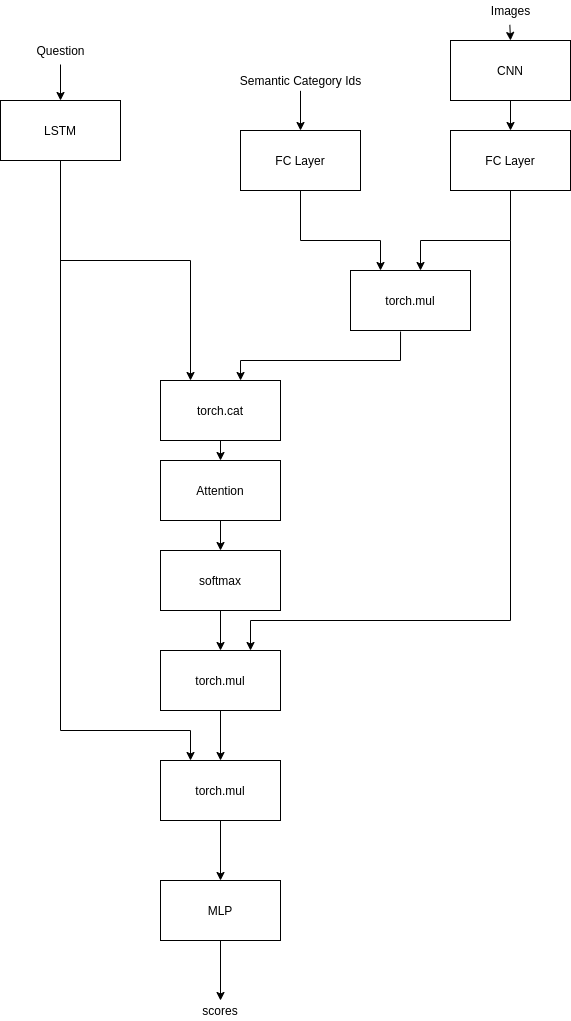
\includegraphics[width=.5\textwidth]{/home/yasmeen/Desktop/thesisproj/thesis/figure/model_w_semantic.png}
     \caption{Model With Semantic Category IDs as 3rd input}
     \label{fig:category_model}
\end{figure}
